\documentclass[11pt]{article}
\usepackage{geometry}                
\geometry{a4paper,left=2.5cm,right=2.5cm,top=2.5cm,bottom=2.5cm}
\usepackage{natbib}
\usepackage{color}
\definecolor{mygreen}{RGB}{28,172,0} % color values Red, Green, Blue
\definecolor{mylilas}{RGB}{170,55,241}
\usepackage{epsfig}
\usepackage{amssymb,amsmath}
\usepackage{enumerate}
\usepackage{enumitem}
\usepackage[utf8]{inputenc}
\usepackage{hyperref}
\usepackage{mathtools}


\newcommand{\ssd}{\text{ssd}}
\newcommand{\sS}{\mathsf{S}}
\newcommand{\tot}{\text{tot}}

\usepackage[procnames]{listings}
\usepackage{color}

\begin{document}

\definecolor{keywords}{RGB}{255,0,90}
\definecolor{comments}{RGB}{0,0,113}
\definecolor{red}{RGB}{160,0,0}
\definecolor{green}{RGB}{0,150,0}

\lstset{language=Python, 
        basicstyle=\ttfamily\small, 
        keywordstyle=\color{keywords},
        commentstyle=\color{comments},
        stringstyle=\color{red},
        showstringspaces=false,
        identifierstyle=\color{green},
        procnamekeys={def,class}}
 

\newcommand{\com}{\, ,}
\newcommand{\per}{\, .}

%% Averages
% Use \bar to over line solo symbols

\newcommand{\av}[1]{\bar{#1}}
\newcommand{\avbg}[1]{\overline{#1}}
\newcommand{\avbgg}[1]{\overline{#1}}

% A nice definition
\newcommand{\defn}{\ensuremath{\stackrel{\mathrm{def}}{=}}}

% space in equations
\newcommand{\qqand}{\qquad \text{and} \qquad}
\newcommand{\qand}{\quad \text{and} \quad}

% equations
\def\beq{\begin{equation}}
\def\eeq{\end{equation}}

\def\bea{\begin{align}}
\def\ena{\end{align}}


% calculus
\newcommand{\ord}{\mathcal{O}}
\newcommand{\p}{\partial}
\newcommand{\ii}{{\rm i}}
\newcommand{\dd}{{\rm d}}
\newcommand{\id}{{\, \rm d}}
\newcommand{\ee}{{\rm e}}
\newcommand{\DD}{{\rm D}}
\newcommand{\wavy}{\text{wavy}}
\newcommand{\qg}{\text{qg}}
\newcommand{\dt}{\Delta t}
\newcommand{\dx}{\Delta x}
\newcommand{\be}{\beta}

\newcommand{\al}{\alpha}
\newcommand{\bx}{\boldsymbol{x}}
\newcommand{\by}{\boldsymbol{y}}
\newcommand{\bu}{\boldsymbol{u}}
\newcommand{\bv}{\boldsymbol{v}}


\newcommand{\half}{\tfrac{1}{2}}
\newcommand{\halfrho}{\tfrac{1}{2}}
\newcommand{\rz}{{}}
\newcommand{\bn}{\boldsymbol{\hat n}}
\newcommand{\br}{\boldsymbol{r}}
\newcommand{\bR}{\boldsymbol{R}}
\newcommand{\bA}{\ensuremath {\boldsymbol {A}}}
\newcommand{\bB}{\ensuremath {\boldsymbol {B}}}
\newcommand{\bU}{\ensuremath {\boldsymbol {U}}}
\newcommand{\bE}{\ensuremath {\boldsymbol {E}}}
\newcommand{\bN}{\ensuremath {\boldsymbol {\mathrm{N}}}}
\newcommand{\bJ}{\ensuremath {\boldsymbol {J}}}
\newcommand{\bXX}{\ensuremath {\boldsymbol {\mathcal{X}}}}
\newcommand{\bFF}{\ensuremath {\boldsymbol {F}}}
\newcommand{\bF}{\ensuremath {\boldsymbol {F}^{\sharp}}}
\newcommand{\bG}{\ensuremath {\boldsymbol G}}
\newcommand{\bSigma}{\ensuremath {\boldsymbol {\Sigma}}}
\newcommand{\bvarphi}{\ensuremath {\boldsymbol {\varphi}}}
\newcommand{\bxi}{\ensuremath {\boldsymbol {\xi}}}
\newcommand{\avbxi}{\overline{\ensuremath {\boldsymbol {\xi}}}}

% math cal

\newcommand{\J}{\mathcal{J}}
\newcommand{\K}{\mathcal{K}}
\newcommand{\cG}{\mathcal{G}}
\newcommand{\cF}{\mathcal{F}}
\newcommand{\cN}{\mathcal{N}}
\newcommand{\cL}{\mathcal{L}}


% san serif for matrices and differential operators
%\newcommand{\helmn}{\mathsf{H}_n}
\newcommand{\helmm}{\triangle_m}
\newcommand{\helmn}{\triangle_n}
\newcommand{\helms}{\triangle_s}
\newcommand{\helm}{\triangle}
\newcommand{\sA}{\mathsf{A}}
\newcommand{\sB}{\mathsf{B}}
\newcommand{\sG}{\mathsf{G}}
\newcommand{\sI}{\mathsf{I}}
\newcommand{\sJ}{\mathsf{J}}
\newcommand{\gsJ}{\breve{\mathsf{J}}}
\newcommand{\sU}{\mathsf{U}}
\newcommand{\sP}{\mathsf{P}}
\newcommand{\sQ}{\mathsf{Q}}
\newcommand{\sR}{\mathsf{R}}
\newcommand{\sL}{\mathsf{L}}
\newcommand{\Lu}{\mathsf{L}(\what{u}_k)}
\newcommand{\Nu}{\mathsf{N}(\what{u}_k)}
\renewcommand{\L}{\mathsf{L}}
\newcommand{\N}{\mathsf{N}}
\newcommand{\sH}{\mathsf{H}}
\renewcommand{\sJ}{\mathsf{J}}
\renewcommand{\sI}{\mathsf{I}}
\renewcommand{\L}{\mathsf{L}}
\newcommand{\sM}{\mathsf{M}}
\newcommand{\sT}{\mathsf{T}}
\newcommand{\sGamma}{\mathsf{\Gamma}}
\newcommand{\sOmega}{\mathsf{\Omega}}
\newcommand{\sSigma}{\mathsf{\Omega}}
\newcommand{\sbeta}{\mathsf{\beta}}
\newcommand{\sPi}{\mathsf{\Pi}}
\newcommand{\sC}{\mathsf{C}}
\newcommand{\sQy}{\mathsf{Q}}
\renewcommand{\sb}{\mathsf{b}}

% u
\newcommand{\uhat}{\what{u}_k}

% angle brackets

\def\la{\langle}
\def\ra{\rangle}
\def\laa{\left \langle}
\def\raa{\right \rangle}


%grads and div's
\newcommand{\bcdot}{\hspace{-0.1em} \boldsymbol{\cdot} \hspace{-0.12em}}
\newcommand{\bnabla}{\boldsymbol{\nabla}}
\newcommand{\bnablaH}{\bnabla_{\! \mathrm{h}}}
\newcommand{\grad}{\bnabla}
\newcommand{\gradH}{\bnablaH}
\newcommand{\curl}{\bnabla \!\times\!}
\newcommand{\diver}{\bnabla \bcdot }
\newcommand{\cross}{\times}
\newcommand{\lap}{\nabla^2}


%varthetas and thetas
\newcommand{\vth}{\vartheta}
\newcommand{\psii}{\psi^{\mathrm{i}}}
\newcommand{\thb}{\theta^{\mathrm{-}}}
\newcommand{\vthb}{\vartheta^{\mathrm{-}}}
\newcommand{\vthbhat}{{\hat{\vartheta}}^{\mathrm{-}}}
\newcommand{\vThb}{\varTheta^{\mathrm{-}}}
\newcommand{\psib}{\psi^{\mathrm{-}}}
\newcommand{\tht}{\theta^{\mathrm{+}}}
\newcommand{\vtht}{\vartheta^{\mathrm{+}}}
\newcommand{\vththat}{{\hat{\vartheta}}^{\mathrm{+}}}
\newcommand{\vthtbhat}{{\hat{\vartheta}}^{\pm}}
\newcommand{\vTht}{\varTheta^{\mathrm{+}}}
\newcommand{\vthtb}{\vartheta^{\pm}}
\newcommand{\vThtb}{\varTheta^{\pm}}

% nondimensional numbers
\renewcommand{\Re}{\mathrm{Re}}
\newcommand{\Ro}{\mathrm{Ro}}
\newcommand{\Ri}{\mathrm{Ri}}

%psi's
%Galerking coefficient for psi:
\newcommand{\gpsi}{\breve \psi}
\newcommand{\gpsic}{{\breve \psi}^\star}
\newcommand{\gtau}{\breve \tau}
\newcommand{\gtauc}{{\breve \tau}^\star}
\newcommand{\gphi}{\breve \phi}
\newcommand{\gq}{\breve q}
\newcommand{\gU}{\breve U}
\newcommand{\gQ}{\breve Q}
\newcommand{\gsigma}{\breve \sigma}


\newcommand{\psit}{\psi^{\mathrm{+}}}
\newcommand{\psithat}{{\hat{\psi}}^{\mathrm{+}}}
\newcommand{\psibhat}{{\hat{\psi}}^{\mathrm{-}}}
\newcommand{\psitb}{\psi^{\pm}}
\newcommand{\psitbhat}{{\hat{\psi}}^\pm}
\newcommand{\St}{S^{\mathrm{+}}}
\newcommand{\Sb}{S^{\mathrm{-}}}
\newcommand{\phb}{\phi^{\mathrm{-}}}
\newcommand{\pht}{\phi^{\mathrm{+}}}
\newcommand{\tautb}{\tau^{\pm}}
\newcommand{\sigmatb}{\sigma^{\pm}}


\newcommand{\bur}{\left(\tfrac{f_0}{N}\right)^2}
\newcommand{\ibur}{\left(\tfrac{N}{f_0}\right)^2}
\newcommand{\Nm}{N_{\mathrm{mix}}}
\newcommand{\xim}{\xi_{\mathrm{mix}}}
\newcommand{\hs}{h_*}
\renewcommand{\sp}{\mathsf{p}}
\newcommand{\se}{\mathsf{e}}
\newcommand{\sptb}{\mathsf{p}^\pm}


%nmax is a problem:
%\newcommand{\nmax}{n_{\mathrm{max}}}
\newcommand{\nmax}{\mathrm{N}}
\newcommand{\mmax}{\mathrm{M}}

\newcommand{\WKB}{\mathrm{WKB}}
\newcommand{\Lam}{\Lambda}
\newcommand{\tha}{\theta}
\newcommand{\kap}{\kappa}
\newcommand{\bphi}{\boldsymbol{\phi}}
\newcommand{\third}{\tfrac{1}{3}}
\newcommand{\cs}{c^\star}
\newcommand{\dstar}{{\star\star}}
\newcommand{\nt}{n^{\mathrm{trnc}}}
\newcommand{\sDp}{\mathsf{D}^1_{\nmax}}
\newcommand{\sDpp}{\mathsf{D}^2_{\nmax}}
\newcommand{\sD}{\mathsf{D}}
\newcommand{\sDN}{\mathsf{D_\nmax}}
\newcommand{\sK}{\mathsf{K_2}}
\newcommand{\stheta}{\mathsf{\theta}}
\newcommand{\sphi}{\mathsf{\phi}}
\newcommand{\sq}{\mathsf{q}}
\newcommand{\cosech}{\text{csch}\,}
\newcommand{\sinc}{\text{sinc}\,}

%%%%%%%%% %%%%
\newcommand{\zp}{z^+}
\newcommand{\zm}{z^-}
\newcommand{\qA}{q^A_{\nmax}}
\newcommand{\psiB}{\psi^B_{\nmax}}
\newcommand{\phiB}{\phi^B_{\nmax}}
\newcommand{\eye}{\boldsymbol{\hat{i}}}
\newcommand{\jay}{\boldsymbol{\hat{j}}}
\newcommand{\kay}{\boldsymbol{\hat{k}}}
\newcommand{\psiG}{\psi^{\mathrm{G}}}
\newcommand{\qG}{q^{\mathrm{G}}}
\newcommand{\uG}{u^{\mathrm{G}}}
\newcommand{\UG}{U^{\mathrm{G}}}
\newcommand{\UGN}{U^{\mathrm{G}}_{\nmax}}
\newcommand{\QGN}{Q^{\mathrm{G}}_{\nmax}}
\newcommand{\sumoddn}{\sum_{n = 1, n~ \text{odd}}^{\nmax}}

% bretherton 
\newcommand{\qBr}{q_{\mathrm{Br}}}
\newcommand{\psiBr}{\psi_{\mathrm{Br}}}

\newcommand{\ep}{\epsilon}


\section*{Examples}

\subsection*{Geostrophic Adjustment: 1D and 1L}

In the directory \texttt{src} you will find an example entitled \texttt{example\_1D\_1L\_spectral.py}

First, libraries are imported.  Two standard ones are numpy, for calculations, and matplotlib.pyplot for plotting.  Those are standard to numpy.  Then, there are four other things that are imported:
\begin{itemize}
\item {\bf Steppers} This contains different time-stepping functions.  At the moment we have Euler, Adams-Bashforth 2 (AB2) and Runge-Kutta 4 (RK4).  PyRsw uses adaptive time stepping to try and be more efficient in how the solution is marched forward.
\item {\bf Fluxes} This contains the fluxes for the RSW model.  At the moment there is only the option for a pseudo-spectral model but this will be generalized to include a Finite Volume method as well.
\item {\bf PyRsw} This is the main library and importing Simulation imports the core of the library.  
\item {\bf constants}  This has some useful constants, more can be added if desired.
\end{itemize}

\noindent After the libraries are imported then a simulation object is created.
\begin{lstlisting}
sim = Simulation()
\end{lstlisting}

\noindent  Below specifies the geometry in $x$ and $y$: [Options 'periodic', 'walls']

\noindent We use AB2, a spectral method: [Options: Euler, AB2, RK4]

\noindent We solve the nonlinear dynamics (can be Linear) 

\noindent  Use spectral sw model (no other choices).  Maybe hide this.
\begin{lstlisting}
sim.geomx       = 'walls'            
sim.geomy       = 'periodic'
sim.stepper     = Step.AB2       
sim.method      = 'Spectral'       
sim.dynamics    = 'Nonlinear'    
sim.flux_method = Flux.spectral_sw
\end{lstlisting}

We specify a lot of parameters.  There are some default values that are specified in {\tt PyRsw}.
\begin{lstlisting}
sim.Lx  = 4000e3          # Domain extent               (m)
sim.Ly  = 4000e3          # Domain extent               (m)
sim.geomx = 'periodic'    # Boundary Conditions
sim.geomy = 'periodic'    # Boundary Conditions
sim.Nx  = 128             # Grid points in x
sim.Ny  = 1               # Grid points in y
sim.Nz  = 1               # Number of layers
sim.g   = 9.81            # Gravity                     (m/sec^2)
sim.f0  = 1.e-4           # Coriolis                    (1/sec)
sim.cfl = 0.05            # CFL coefficient             (m)
sim.Hs  = [100.]          # Vector of mean layer depths (m)
sim.rho = [1025.]         # Vector of layer densities   (kg/m^3)
sim.end_time = 36.*hour   # End Time                    (sec)
\end{lstlisting}

We can specify the periodicity of plotting and whether we want a life animation or make a video.  More on this this later.
\begin{lstlisting}
sim.output = False        # True or False
sim.savet  = 1.*hour      # Time between saves
\end{lstlisting}

Specify periodicity of diagnostics and whether to compute them.  This is not tested.
\begin{lstlisting}
sim.diagt    = 2.*minute  # Time for output
sim.diagnose = False      # True or False
\end{lstlisting}

Initialize the simulation.
\begin{lstlisting}
sim.initialize()
\end{lstlisting}

Specify the initial conditions.  There is an option whether we want the domain in $x$ or $y$.  At the moment there is no difference because there is no $\beta$-plane but this will be added.
\begin{lstlisting}
for ii in range(sim.Nz):  # Set mean depths
    sim.soln.h[:,:,ii] = sim.Hs[ii]

# Gaussian initial conditions
x0 = 1.*sim.Lx/2.      # Centre
W  = 200.e3                # Width
amp = 1.                  # Amplitude
if sim.Ny==1:
    sim.soln.h[:,:,0] += amp*np.exp(-(sim.x-x0)**2/(W**2)).reshape((sim.Nx,1))
elif sim.Nx==1:
    sim.soln.h[:,:,0] += amp*np.exp(-(sim.y-x0)**2/(W**2)).reshape((1,sim.Ny))
\end{lstlisting}

Solve the problem.
\begin{lstlisting}
sim.run()             
\end{lstlisting}

Plot the Hovm\"oller diagram in time versus space.
\begin{lstlisting}
if sim.Ny==1:
    plt.figure               
    t = np.arange(0,sim.end_time+sim.plott,sim.plott)/86400.
        
    for L in range(sim.Nz):
        field = sim.hov_h[:,0,:].T - np.sum(sim.Hs[L:])
        plt.subplot(sim.Nz,1,L+1)
        plt.pcolormesh(sim.x/1e3,t, field,
            cmap=sim.cmap, vmin = 0, vmax = amp)
        plt.xlim([sim.x[0]/1e3, sim.x[-1]/1e3])
        plt.ylim([t[0], t[-1]])
        plt.title(r"$Hovm{\"o}ller Plot\, {of} \,\, \eta$")
        plt.xlabel(r"$distance \, \, (km)$")
        plt.ylabel(r"$Time \, \, (days)$")
        plt.colorbar()
    plt.show()
\end{lstlisting}

\begin{figure}[h]
\begin{center}
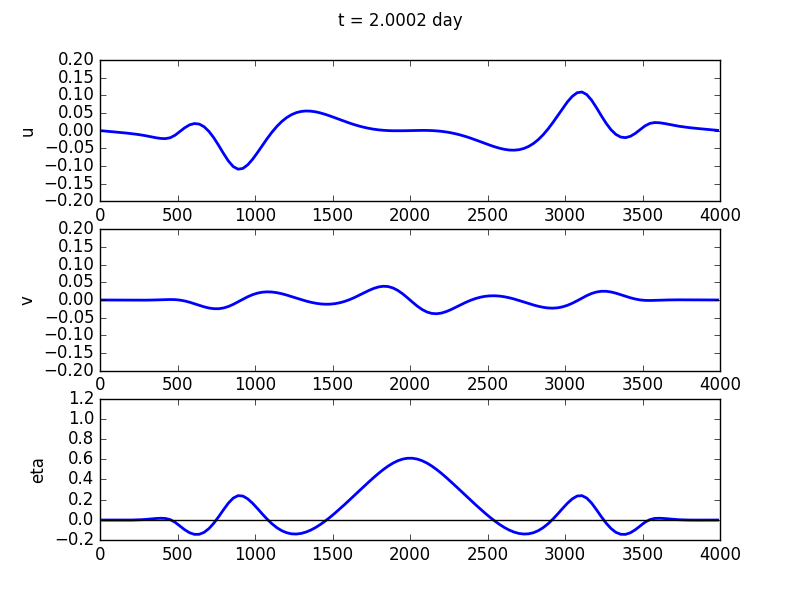
\includegraphics[width=12cm]{Figures/ex1_fig1.png}
\caption{Final solution for the test case.}
\end{center}
\end{figure}

\begin{figure}[h]
\begin{center}
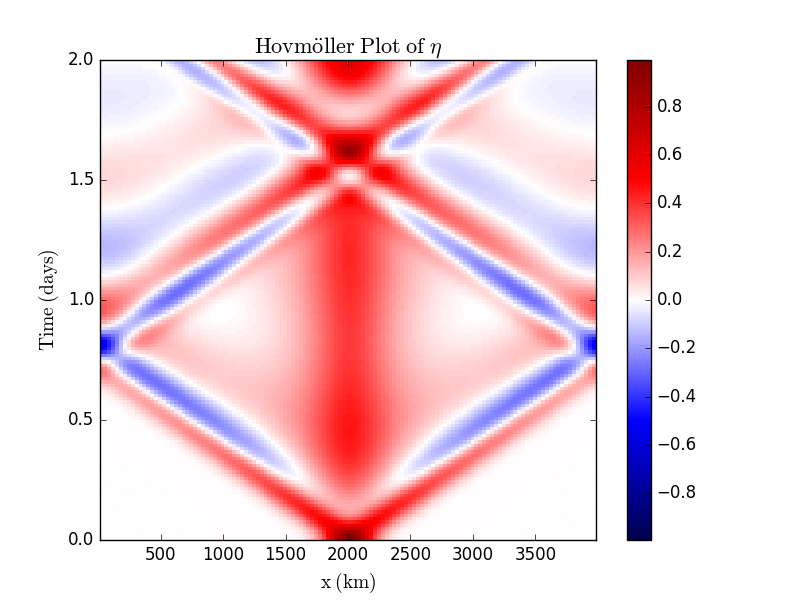
\includegraphics[width=12cm]{Figures/ex1_fig2.png}
\caption{Hovm\"oller plot for the test case.}
\end{center}
\end{figure}

There is a second example called {\tt example\_1D\_geoadjust2.py} that begins with a hyperbolic tangent profile instead if a Gaussian initial condition.

\subsection*{Geostrophic Adjustment: 2D and 1L}

The basic script is almost identical to the 1D case.  The changes are as follows:
\begin{itemize}
\item[1.] Set $Nx$ and $Ny$ both equal to $128$, and from this we build a 2D grid.   
\item[2.] Define the initial conditions on a 2D grid.
\item[3.] The plotting is different.  We plot a 2D field using \tt{pcolormesh} and we don't do a Hovm\"oller plot.
\end{itemize}

\subsection*{Bickley Jet: 2D and 1L}

Following Poulin and Flierl (2003) and Irwin and Poulin (2014), we look at the instability of a jet.
\end{document}